By using multiple robots the possibilities are expanded but under certain conditions, such as, they do not interfere with each other and do not redo the work of others. For exploration it means that they have to know where the others are or have been, in order to do that the robots need to merge their map to identify their common or uncommon environments.\\
This problem can be represented as a graph where the nodes are the positions of the robots at a certain time and the arcs are the transformation matrix from a node to another:

\begin{figure}[H]
\centering
    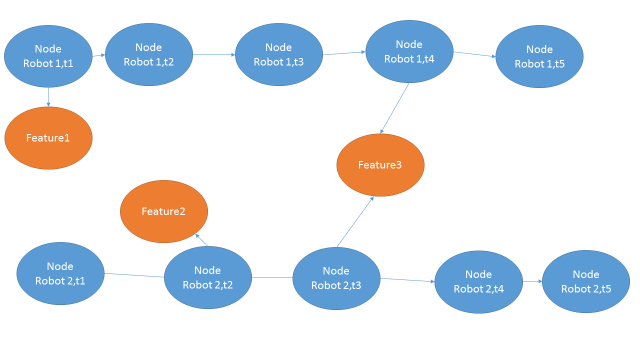
\includegraphics[scale=0.6]{graphslam.png} 
    \caption{Graph representation of the Multi-robot SLAM problem.}
    \label{fig:difalgo}
\end{figure}

The goal of this problem is to make the link between robot 1 and robot 2 (with the feature 3 in figure 9) of course in some contexts a sole link between the graphs would not be sufficient (with sensors getting only range), and would need two or three links two associate the graph.
Another method would be to iterate over each feature from the graph of a robot and try to match it to the features of another graph, it is the same reasoning as the ICP (Iterative Closest Point) method use for matching frames for a 3D mapping.
